\documentclass[a4paper, 11pt]{article}
\usepackage[utf8]{inputenc}
\usepackage[german]{babel}
\usepackage[T1]{fontenc}
\usepackage{datetime}
\usepackage{textcomp}
\usepackage{listings}
\usepackage[usenames,dvipsnames]{color}
\usepackage[margin=.7in,lmargin=1in]{geometry}
\usepackage{fancyhdr}
\usepackage{lastpage}
\usepackage[colorlinks=true,urlcolor=blue,linkcolor=blue]{hyperref} 
\usepackage{upquote}
\usepackage[scaled=1]{beramono}
\setlength{\parindent}{0pt}
\usepackage{graphicx}
\usepackage[inline]{enumitem}

\def\shortyear#1{\expandafter\shortyearhelper#1}
\def\shortyearhelper#1#2#3#4{#3#4}
\newdateformat{specialdate}{\shortyear{\the\year}.\twodigit{\THEMONTH}.\twodigit{\THEDAY}}
\renewcommand{\headrulewidth}{0pt}
\pagestyle{fancy}
\lhead{}

\date{\vspace{-5ex}}
\chead{}
\rhead{}
\lfoot{LÖVE Spieleprogrammierung - \date{\specialdate\today}}
\cfoot{\thepage/\pageref*{LastPage}}
\rfoot{\href{http://espws.de}{espws.de}}
\definecolor{darkgray}{rgb}{0.45, 0.45, 0.45}
\definecolor{lightgray}{rgb}{0.9, 0.9, 0.9}

\lstdefinestyle{colorstyle}
{
  numbers          = left,
  language         = {[5.2]Lua},
  basicstyle       = \ttfamily,
  showstringspaces = false,
  commentstyle     = \itshape\color{darkgray},
  numberstyle      = \tiny,
  identifierstyle  = \color{blue},
  keywordstyle     = \color{magenta},
  stringstyle      = \color{red},
  xleftmargin      = 0em,
  rulecolor        = \color{lightgray},
  frame            = l,
  framexleftmargin = .2em
}

\title{\vspace{-8ex}Einstieg Spiele-Programmierung in LÖVE\vspace{-1ex}}

\author{\copyright{} 2016 Iwan Gabovitch (\href{http://espws.de}{espws.de})\\
Lizenziert unter einer \href{http://creativecommons.org/licenses/by-sa/4.0/}{Attribution-ShareAlike 4.0 International Lizenz}}

\lstset{
  style              = colorstyle,
  escapeinside       = {\%*}{*)},
  breaklines         = true,
  breakatwhitespace  = true,
  framextopmargin    = 2pt,
  framexbottommargin = 2pt,
  inputencoding      = utf8,
  extendedchars      = true,
  literate           = {ä}{{\"a}}1 {Ä}{{\"A}}1 {ö}{{\"o}}1 {Ö}{{\"O}}1 {ü}{{\"u}}1 {Ü}{{\"U}}1 {ß}{{\ss}}1,
}

\exhyphenpenalty=10000\hyphenpenalty=10000
\widowpenalty=10000
\raggedbottom
\clubpenalty=10000
\sloppy

\begin{document}

\maketitle
\thispagestyle{fancy}

\begin{center}
  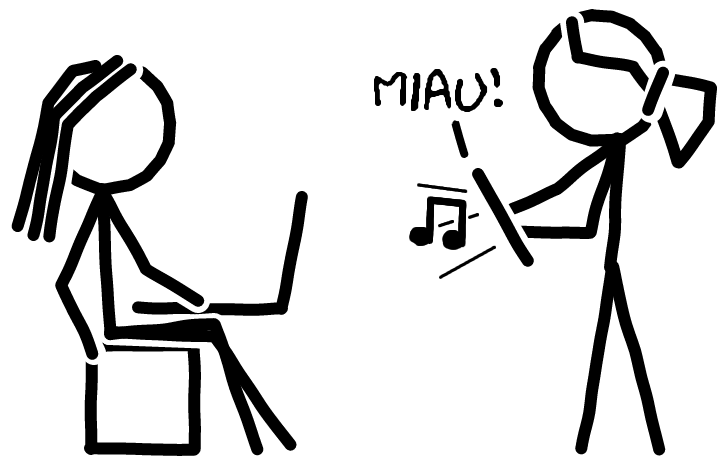
\includegraphics[width=.4\textwidth]{graphics/fertig.png}
\end{center}

\section{Vorbereitung}

\begin{enumerate}
  \item Extrahiere \textbf{StartGamedev} und öffne den Texteditor mithilfe der \texttt{open-editor} Datei.
  \item Lese Aufgaben aufmerksam, tippe Code (\textit{Quelltext}) ab und teste Ergebnisse.
\end{enumerate}

\section{Miau Spiele-App}

\subsection{Interaktiver Sound}

\textbf{Tippe} den folgenden Code \textbf{ab}, speichere und teste diesen:

\lstinputlisting{code/1all1.lua}

Der Code in \texttt{love.load()} lädt eine Sounddatei und \texttt{love.mousepressed()} spielt diese ab, wenn ein Mausknopf gedrückt oder der Touchscreen berührt wird.

\subsection{Interaktive Bilder}

\textbf{Ergänze} \texttt{love.load()} mit dem Laden zweier Bilder:

\lstinputlisting{code/1load2de.lua}

\textbf{Füge} folgende zwei Funktionen zu Deinem Code \textbf{hinzu}:

\lstinputlisting{code/1add2de.lua}

\texttt{love.update()} berechnet, welches der Bilder das aktuelle ist. \texttt{love.draw()} zeichnet dieses. Beide Funktionen arbeiten 60 mal je Sekunde. Das Bild passt nicht ganz aber darum kümmern wir uns später.

\subsection{Zufällige Miau Sounds}

\textbf{Ergänze} \texttt{love.load()} mit folgender Liste bzw. Tabelle an Sounds:

\lstinputlisting{code/1load3de.lua}

\textbf{Ersetze} den Inhalt von \texttt{love.update()} mit Code, welcher die Soundliste benutzt:

\lstinputlisting{code/1update3de.lua}

\textbf{Ersetze} den Inhalt von \texttt{love.mousepressed()} mit Code, welcher zufällige Sounds abspielt:

\lstinputlisting{code/1mousepressed3de.lua}

\subsection{Anpassung an verschiedene Bildschirme}

\textbf{Ergänze} den Inhalt von \texttt{love.load()} mit Berechnungen der Verhältnisse der Fenster- zu Bildgrößen:

\lstinputlisting{code/1load4.lua}

\textbf{Ergänze} den \texttt{love.graphics.draw()} Funktionsaufruf in \texttt{love.draw()} mit Skalier-Parametern:

\lstinputlisting{code/1draw4de.lua}

Das Bild wird dadurch an die Bildschirmgröße angepasst skaliert dargestellt, da Handys/Tablets nur eine Auflösung unterstützen. Dies ist zwar nicht optimal aber eine einfache Lösung für den Anfang.

\subsection{Android-Port} \label{androidport}

Du kannst eigene Grafiken (am Computer oder auf Papier gemalt) oder eigene Sounds in Deine Miau Spiele-App einzubauen und das App-Icon ändern.

Wir empfehlen zu programmieren, dass der "`Zurück"'-Knopf die Android-App schließt:

\lstinputlisting{code/1keypressed5.lua}

Um die App auf Android spielbar zu machen, muss ein Zip-Archiv von dem Spiel erstellt werden, in \texttt{game.love} umbenannt werden und ins \texttt{StartGamedev}-Verzeichnis gelegt werden. Dann muss das \texttt{make-apk} Skript benutzt werden. Die resultierende \texttt{game.apk} muss dann aufs Handy/Tablet kopiert und dort installiert werden.

\newpage

\section{Katz und Maus Spiele-App}

\subsection{Bild und Sound}

\textbf{Tippe} den folgenden Code \textbf{ab} (ohne \texttt{-{}- Kommentare}), speichere und teste diesen:

\lstinputlisting{code/2all1de.lua}

Der Code in \texttt{love.load()} verändert die Fensterauflösung, lädt Bilder und Musik, setzt Positions-Variablen und spielt die Musik. \texttt{love.draw()} malt die Bilder, 60 mal je Sekunde. Sie passen nicht ganz aber darum kümmern wir uns später.

\newpage

\subsection{Automatische und Interaktive Bewegung}

\textbf{Ergänze} \texttt{love.load()} mit Mausklick-Positions-Variablen und Sounds:

\lstinputlisting{code/2load2de.lua}

\textbf{Füge} folgende drei Funktionen zu Deinem Code \textbf{hinzu}:

\lstinputlisting{code/2add2de.lua}

Die Funktion \texttt{distanz()} berechnet den Abstand zwischen zwei Punkten mithilfe des Satzes des Pythagoras bzw. der Formel $c = \sqrt{a^2 + b^2}$.

\texttt{love.update()}
\begin{enumerate*}
  \item Bewegt die Maus,
  \item Setzt die Maus zurück, wenn sie über den rechten Rand läuft oder
  \item wenn Katze und Maus sich berühren,
  \item Bewegt die Katze.
\end{enumerate*}

Der Code in \texttt{love.mousepressed()} verändert die \texttt{klickX} und \texttt{klickY} Variablen jedes Mal, wenn ein Mausknopf oder der Touchscreen berührt wird.

\newpage

\subsection{Bildschirmgröße}

\textbf{Ergänze} den Inhalt von \texttt{love.load()} mit Berechnungen der Verhältnisse der Fenster- zu Bildgrößen:

\lstinputlisting{code/2load3.lua}

\textbf{Ergänze} die \texttt{love.graphics.draw()} Funktionsaufrufe in \texttt{love.draw()} mit Skalier-Parametern:

\lstinputlisting{code/2draw3de.lua}

\textbf{Ersetze} die Variablenzuweisungen in \texttt{love.mousepressed()}, um vom Bildschirm aufs Spielefeld zu projezieren:

\lstinputlisting{code/2mousepressed3de.lua}

\subsection{Punkte und Zeit}

\textbf{Ergänze} den Inhalt von \texttt{love.load()} mit Bildgrößen, Schrift-Einstellung, Zeit und Punkten:

\lstinputlisting{code/2load4de.lua}

\textbf{Ergänze} den Inhalt von \texttt{love.update()} mit einer Zeitberechnung:

\lstinputlisting{code/2update4ade.lua}

\textbf{Ergänze} den \texttt{if}-Block in \texttt{love.update()}, der auf Katz-Maus Berührungen reagiert, mit einer Punkte-Hochrechnung:

\lstinputlisting{code/2update4bde.lua}

\textbf{Ergänze} den Inhalt von \texttt{love.draw()}, sodass Zeit und Punkte angezeigt werden:

\lstinputlisting{code/2draw4de.lua}

Du solltest den Inhalt von \texttt{love.update()} in einen \colorbox{lightgray}{\texttt{if zeit > 0 then ... end}}-Block packen, um das Spiel nach Zeitablauf anzuhalten. Du kannst einen ähnlichen Block in \texttt{love.draw()} verwenden, um eine "`Game Over!"' Nachricht anzuzeigen.

\newpage

\section{Matrix-Musik DJ-App}

\textbf{Tippe} den folgenden Code \textbf{ab} (ohne \texttt{-{}- Kommentare}), speichere und teste diesen:

\lstinputlisting{code/3all1de.lua}

Der Code macht intensiven Gebrauch von Tabellen/Listen und \texttt{for}-Schleifen, sowie von mathematischen Berechnungen, die etwas langsamer verdaut werden sollten.

\end{document}
